\section{Makna Geometris Perkalian Skalar}

\begin{outcome}

\begin{enumerate}

\item[A.] Memahami perkalian skalar secara geometris.

\end{enumerate}
\end{outcome}

Ingat bahwa titik $P=\left( p_{1},p_{2},p_{3}\right) $ menentukan
sebuah vektor $\vect{p}$ dari $0$ ke $P$. Panjang $\vect{p}$, yang dinyatakan dengan $\vectlength
\vect{p} \vectlength $, sama dengan $
\sqrt{p_{1}^{2}+p_{2}^{2}+p_{3}^{2}}$ berdasarkan Definisi \ref{def:distancebetweenpoints}.

Sekarang misalkan kita memiliki vektor $\vect{u} = \leftB
\begin{array}{lll}
u_1 &  u_2 & u_3
\end{array}
\rightB^T$ dan kita mengalikan $\vect{u}$ dengan suatu
skalar $k$. Berdasarkan Definisi \ref{def:vectorscalarmultiplication},
$k\vect{u} = \leftB
\begin{array}{rrr}
ku_{1} & ku_{2} & ku_{3}
\end{array}
\rightB^T $.
Kemudian, dengan menggunakan Definisi \ref{def:distancebetweenpoints}, panjang vektor ini diberikan oleh
\begin{equation*}
\sqrt{\left( \left( k u_{1}\right) ^{2}+\left( k u_{2}\right)
^{2}+\left( k u_{3}\right) ^{2}\right) }=\left\vert k \right\vert
\sqrt{u_{1}^{2}+u_{2}^{2}+u_{3}^{2}}
\end{equation*}
Jadi, hubungan berikut berlaku.
\begin{equation*}
\vectlength k \vect{u} \vectlength =\left\vert k \right\vert
\vectlength \vect{u} \vectlength
\end{equation*}
Dengan kata lain, perkalian dengan suatu skalar memperbesar atau memperkecil panjang
vektor dengan faktor $\left\vert k \right\vert$. Jika $\left\vert k \right\vert > 1$, panjang vektor yang dihasilkan akan
diperbesar. Jika $\left\vert k \right\vert <1$, panjang vektor yang dihasilkan akan menyusut. Ingat bahwa berdasarkan definisi
nilai mutlak, $\left\vert k \right\vert >0$.

Bagaimana dengan arahnya? Gambarkan $\vect{u}$ dan $k\vect{u}$
ketika $k$ negatif. Perhatikan bahwa hal ini menyebabkan vektor yang dihasilkan
menunjuk ke arah yang berlawanan, sedangkan jika $k >0$, arah hadap
vektor tetap dipertahankan. Oleh karena itu, arah dapat berbalik
jika $k < 0$, atau tetap dipertahankan jika $k > 0$.

Perhatikan contoh berikut.

\begin{example}{Menggambar Perkalian Skalar}\label{exa:graphingscalarmult}
Perhatikan vektor $\vect{u}$ dan $\vect{v}$ yang digambar di bawah ini.

\begin{center}
\begin{tikzpicture}[scale=2]
\draw[->, thick, blue] (0,0)--(2,1);
\draw[->, thick, red] (4,1)--(5,0.5);
\node[below] at (1,1.25){$\vect{u}$};
\node[above right] at (4.5, 0.75){$\vect{v}$};
\end{tikzpicture}\par\captionof{figure}{Sketsa dua dimensi vektor u (biru, ke atas dan ke kanan) serta v (merah, ke bawah dan ke kanan) yang digambar sebagai...}\label{fig:RnVectorsScalarMultMeaning-tikz01}% fig-num-auto

\end{center}

Gambarkan $-\vect{u}$, $2\vect{v}$, dan $-\frac{1}{2}\vect{v}$.
\end{example}

\begin{solution}

Untuk menemukan $-\vect{u}$, kita mempertahankan panjang $\vect{u}$ dan cukup membalik arahnya.
Untuk $2\vect{v}$, kita menggandakan panjang $\vect{v}$ sambil mempertahankan arahnya. Terakhir,
$-\frac{1}{2}\vect{v}$ diperoleh dengan mengambil setengah panjang $\vect{v}$ dan membalik arahnya.
Vektor-vektor ini ditunjukkan dalam diagram berikut.

\begin{center}
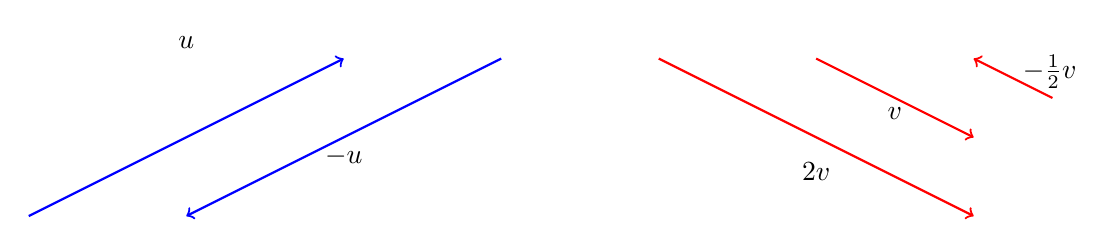
\begin{tikzpicture}[scale=2]
\draw[->, thick, blue] (0,0)--(2,1);
\draw[->, thick, blue] (3,1)--(1,0);
\draw[->, thick, red] (5,1)--(6,0.5);
\draw[->, thick, red] (6.5,0.75)--(6,1);
\draw[->, thick, red] (4,1)--(6,0);
\node[above] at (1,1){$\vect{u}$};
\node[below] at (2,0.5){$-\vect{u}$};
\node[below] at (5.5, 0.75){$\vect{v}$};
\node[above right] at (6.25, 0.75){$-\frac{1}{2}\vect{v}$};
\node[below] at (5, 0.4){$2\vect{v}$};
\end{tikzpicture}\par\captionof{figure}{Diagram dua dimensi yang menunjukkan kelipatan skalar dua vektor: vektor u berwarna biru dan negatifnya -u...}\label{fig:RnVectorsScalarMultMeaning-tikz02}% fig-num-auto

\end{center}

\end{solution}

Setelah mempelajari penjumlahan vektor dan perkalian skalar, sekarang kita dapat menggabungkan kedua tindakan tersebut. Ingat
Definisi \ref{def:linearcombination} mengenai kombinasi linear matriks kolom. Kita dapat menerapkan definisi ini pada
vektor dalam $\mathbb{R}^n$. Kombinasi linear vektor dalam $\mathbb{R}^n$ adalah jumlah vektor-vektor yang dikalikan dengan skalar.

Dalam contoh berikut, kita mengkaji makna geometris konsep ini.

\begin{example}{Menggambar Kombinasi Linear Vektor}\label{exa:graphinglinearcombination}
Perhatikan gambar vektor $\vect{u}$ dan $\vect{v}$ berikut.

\begin{center}
\begin{tikzpicture}[scale=2]
\draw[->, thick, blue] (0,0)--(2,1);
\draw[->, thick, red] (4,1)--(5,0.5);
\node[below] at (1,1.25){$\vect{u}$};
\node[above right] at (4.5, 0.75){$\vect{v}$};
\end{tikzpicture}\par\captionof{figure}{Sketsa dua dimensi vektor u (biru, ke atas dan ke kanan) serta v (merah, ke bawah dan ke kanan) yang digambar sebagai...}\label{fig:RnVectorsScalarMultMeaning-tikz03}% fig-num-auto

\end{center}

Buatlah sketsa $\vect{u}+2\vect{v},\vect{u}-\frac{1}{2}\vect{v}.$
\end{example}

\begin{solution}
Kedua vektor tersebut ditunjukkan di bawah ini.

\begin{center}
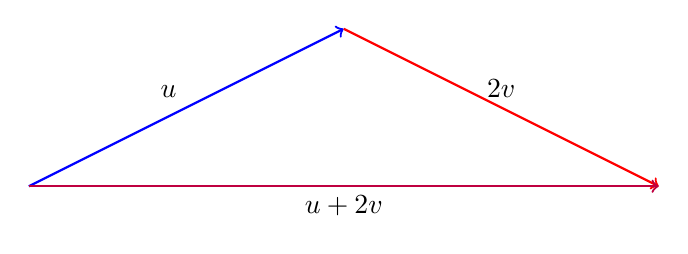
\begin{tikzpicture}[scale=2]
\draw[->, thick, blue] (0,0)--(2,1);
\draw[->, thick, red] (2,1)--(4,0);
\draw[->, thick, purple](0,0)--(4,0);
\node[above left] at (1,0.5){$\vect{u}$};
\node[above] at (3,0.5){$2\vect{v}$};
\node[below] at (2,0){$\vect{u}+2\vect{v}$};
\end{tikzpicture}\par\captionof{figure}{Diagram vektor dua dimensi untuk kombinasi linear u + 2v: vektor u berwarna biru dari titik asal, berwarna merah...}\label{fig:RnVectorsScalarMultMeaning-tikz04}% fig-num-auto

\end{center}
\begin{center}
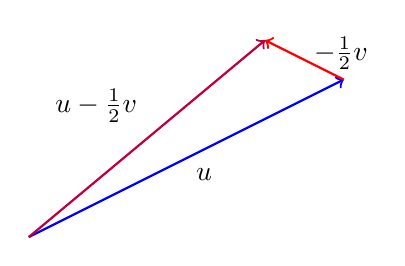
\begin{tikzpicture}[scale=2]
\draw[->, thick, blue] (0,0)--(2,1);
\draw[->, thick, red] (2,1)--(1.5, 1.25);
\draw[->, thick, purple](0,0)--(1.5,1.25);
\node[below right] at (1,0.5){$\vect{u}$};
\node[above right] at (1.75,1){$-\frac{1}{2}\vect{v}$};
\node[below left] at (0.75, 1){$\vect{u} - \frac{1}{2}\vect{v}$};
\end{tikzpicture}\par\captionof{figure}{Diagram vektor dua dimensi untuk kombinasi linear u - 1/2 v: u berwarna biru dari titik asal, lalu...}\label{fig:RnVectorsScalarMultMeaning-tikz05}% fig-num-auto

\end{center}
\end{solution}
